% Copyright (c) 2008-2009 solAvethis
% Copyright (c) 2010-2016,2018 Casper Ti. Vector
% Copyright (c) 2020-2021 jiafeng5513
% Copyright (c) 2025-2026 liupy8222
% Public domain.Aa

% 默认为书籍排版即双面打印，openright章节从偶数页开始，openany章节从任意页码开始
% oneside：单面打印   twoside：双面打印

\documentclass[UTF8,oneside,openany,driverfallback=dvipdfmx,pdfencoding=unicode,hidelinks]{jlutex}

\usepackage[perpage]{footmisc}

\usepackage{tikz}
\usetikzlibrary{tikzmark}

\usepackage{multirow}  % 合并行clawhub config set registry https://gitee.com/OpenClaw-CN/clawhub-mirror/raw/main/registry.json
\usepackage{graphicx}  % 调整表格大小
\usepackage{geometry}  % 页面设置
\usepackage{caption}   % 标题设置
\usepackage{float}     % 浮动体控制
\usepackage{makecell} % 用于表头换行
\usepackage{rotating} % 必须添加这个宏包用于横向排版表格

\usepackage{booktabs}
\usepackage{algorithm}
\usepackage{algorithmicx}  
\usepackage{appendix}
\usepackage{algpseudocode}
\usepackage{setspace}

\usepackage[percent]{overpic}

\newcommand*{\rom}[1]{\expandafter (\romannumeral #1)}

\usepackage[backend=biber,style=gb7714-2015, gbnamefmt=lowercase]{biblatex}
\renewcommand*{\bibfont}{\zihao{-5}\linespread{1.25}\selectfont}
% 按学校要求设定参考文献列表的段间距。
\setlength{\bibitemsep}{3bp}


\jlutexinfo{
	cthesisname = {本科毕业论文（设计）},
	ctitle = {扁茎大豆后代稳定品系LFI297的育种可利用性评价}, 
	etitle = {Evaluation of Breeding Utilization of Stable Line LFI297 of Fasciated Stem Soybean Descendants},
	cauthor = {刘鹏宇}, 
	class = {822221},
	studentid = {82220342},
	date = {2026 年 05 月},
	school = {植物科学学院},
	cmajor = {农学}, 
	cmentor = {王英}, mentortitle = {教授},
	ckeywords = {大豆；扁茎；品系；产量}, ekeywords = {Soybean; Fasciated stem; Line; Yield}
}

%++++++++++++++++++++++++++++++++++++++++++++++++++++++
%以下内容尽量不要修改
\addbibresource{ref.bib}	% 载入参考文献数据库（注意不要省略“.bib”）。

\usepackage{color}
% \emergencystretch=2em %边缘距离容差

\makeatletter
\renewcommand{\tableofcontents}{%
	\if@twocolumn
		\@restonecoltrue\onecolumn
	\else
		\@restonecolfalse
	\fi
	\begingroup
		\parindent\z@
		\centering\heiti\zihao{3}\contentsname\par
	\endgroup
	\@mkboth{\contentsname}{\contentsname}%
	\@starttoc{toc}%
	\if@restonecol\twocolumn\fi
}
% 目录字体
\renewcommand{\cftchapfont}{\songti\zihao{4}\bfseries}
\renewcommand{\cftsecfont}{\songti\zihao{4}}
\renewcommand{\cftsubsecfont}{\songti\zihao{4}}

\renewcommand{\cftchappagefont}{\songti\zihao{4}}
\renewcommand{\cftsecpagefont}{\songti\zihao{4}}
\renewcommand{\cftsubsecpagefont}{\songti\zihao{4}}
%给目录中的大章节名后面加上点
\renewcommand{\cftdot}{.}          % 使用点作为引导符 (通常就是默认)
\renewcommand{\cftdotsep}{1}       % 设置点间距
\renewcommand{\cftchapleader}{\cftdotfill{\cftdotsep}}  %章级也加点

\makeatother

%对号和错号
\usepackage{amssymb}% http://ctan.org/pkg/amssymb
\usepackage{pifont}% http://ctan.org/pkg/pifont
\newcommand{\cmark}{\ding{51}}%
\newcommand{\xmark}{\ding{55}}%
%修改全局的表格字号
\usepackage{etoolbox}
\BeforeBeginEnvironment{tabular}{\zihao{-5}}
%表格背景色
\usepackage{colortbl}
% \usepackage{fancyhdr}
\usepackage{arydshln}
\usepackage[nopatch=footnote]{microtype}

\makeatletter
\DeclareFontFamily{OT1}{TimesNewRoman(0)}{}
\DeclareFontShape{OT1}{TimesNewRoman(0)}{m}{n}{<->ssub*lmr/m/n}{}
\DeclareFontShape{OT1}{TimesNewRoman(0)}{m}{it}{<->ssub*lmr/m/it}{}
\DeclareFontShape{OT1}{TimesNewRoman(0)}{b}{n}{<->ssub*lmr/b/n}{}
\DeclareFontShape{OT1}{TimesNewRoman(0)}{b}{it}{<->ssub*lmr/b/it}{}
\makeatother

\defbibheading{bibintoc}{%
  \chapter*{{\zihao{-4}\heiti 参考文献}}%
  \markboth{参考文献}{参考文献}%
  \addcontentsline{toc}{chapter}{参考文献}%
}

\begin{document}{}
	% 以下为正文之前的部分，默认不进行章节编号。
	\frontmatter
	\setcounter{page}{0}		% 重置页码计数器，用大写罗马数字排版此部分页码。\\
	\pagestyle{empty}% 此后到下一 \pagestyle 命令之前不排版页眉或页脚。
	\maketitle					% 生成封面。    
	% 以下三页：扉页 + 原创性声明 + 使用授权声明
	% \innertitle               % 扉页
	% \include{chap/statement}	% 原创性声明
	% \include{chap/copyright}	% 投稿/授权声明
	
	\pagenumbering{Roman}
	\setcounter{page}{1}		% 重置页码计数器，用大写罗马数字排版此部分页码。\\
	\pagestyle{myheading}	% 此后到下一 \pagestyle 命令之前正常排版页眉和页脚。
	\ctexset{chapter={pagestyle=myheading}}

	\begin{cabstract}

		大豆是我国重要的粮油兼作作物，在保障国家植物蛋白与食用油脂安全方面发挥着不可替代的作用。然而，国内大豆单产水平增幅有限，对外依存度居高不下，突破产量瓶颈已成为重大战略任务。扁茎大豆作为形态发生变异的特殊种质资源，因其独特的株型特征（顶端结荚习性、独特茎秆结构）在耐密植育种中展现出巨大潜力，但对其后代稳定品系在不同种植密度下的系统评价相对缺乏，尤其缺乏在产量构成特征及品质稳定性方面的深入研究。

		\end{cabstract}
	
		\begin{eabstract}

		Soybean is a crucial dual-purpose food and oil crop in China, playing an irreplaceable role in ensuring national plant protein and edible oil security. However, the increase in domestic soybean yield remains limited, and foreign dependency continues to be high. Therefore, breaking through the yield bottleneck has become a major strategic task. Fasciated-stem soybean, as a special germplasm resource with morphological variation, shows tremendous potential in dense-planting tolerance breeding due to its unique plant architecture (terminal podding habit and unique stem structure). Nevertheless, there is a relative lack of systematic evaluation of its stable progeny lines under varying planting densities, particularly lacking in-depth research on yield components and quality stability.
	
		Using LFI297, a stable progeny line of fasciated-stem soybean bred by the College of Plant Sciences at Jilin University, consecutive two-year field experiments were conducted in Changchun, Jilin Province, from 2024 to 2025. Different planting density gradients (240,000, 300,000, 340,000, 350,000, 400,000, and 550,000 plants/hm$^2$) were established to systematically investigate the regulatory effects of density on agronomic traits, yield components, and seed quality. Data were analyzed using multiple statistical methods, including analysis of variance (ANOVA), correlation analysis, and principal component analysis (PCA).
		
		\end{eabstract}
	
	
	
	\tableofcontents
	\thispagestyle{myheading}
	\ctexset{chapter={pagestyle=plain}}

	\pagestyle{plain}	% 此后到下一 \pagestyle 命令之前正常排版页眉和页脚。
	\mainmatter% 以下为正文部分，默认要进行章节编号。

	\chapter{前言}

	% 第一层：宏观背景与挑战
	大豆（\textit{Glycine max} (L.) Merr.）起源于中国，是世界范围内最重要的植物蛋白和食用油来源。作为我国核心的粮油兼作作物，大豆在保障国家粮食安全方面发挥着不可替代的战略作用。然而，随着国内消费需求攀升，大豆单产增幅有限，对外依存度居高不下。在耕地面积有限的国情下，通过大豆分子模块设计育种体系、分子设计育种和人工智能育种，培育具有突破性的大豆新品种，增强我国大豆自产能力，缓解大豆需求缺口，已成为我国农业科研的重大战略任务\cite{Tian2018}。
	
	% 第六层：路线图
	本论文的结构安排如下：第二章详细阐述试验材料与田间设计方法；第三章重点剖析种植密度对 LFI297 农艺性状、产量构成及品质的调控效应；第四章结合理想株型理论与本研究结果，深入讨论扁茎大豆后代稳定品系 LFI297 的耐密机理与育种应用价值；第五章总结主要结论并展望未来的研究方向。
	
	
	\chapter{材料与方法}

	\section{试验地概况与气象条件}
	
	本田间试验于 2024 年和 2025 年的 4 月至 10 月期间，在吉林省长春市吉林大学农学部植物科学学院农业教学科研实验基地（43°92′ N, 125°27′ E）开展。该试验区域属于典型的温带大陆性季风气候。2024 年大豆全生育期平均温度为 19.8℃，平均相对湿度为 70\%，总降雨量为 657.5mm，2025 年大豆全生育期平均温度为 20.9℃，平均相对湿度为 68\%，总降雨量为 513.2mm（图~\ref{fig:tianqi}）。土壤类型为典型黑土，地势平坦，排灌方便，基础地力均匀，两年前茬作物均为玉米。
	
	\begin{figure}[htb]
		\centering
		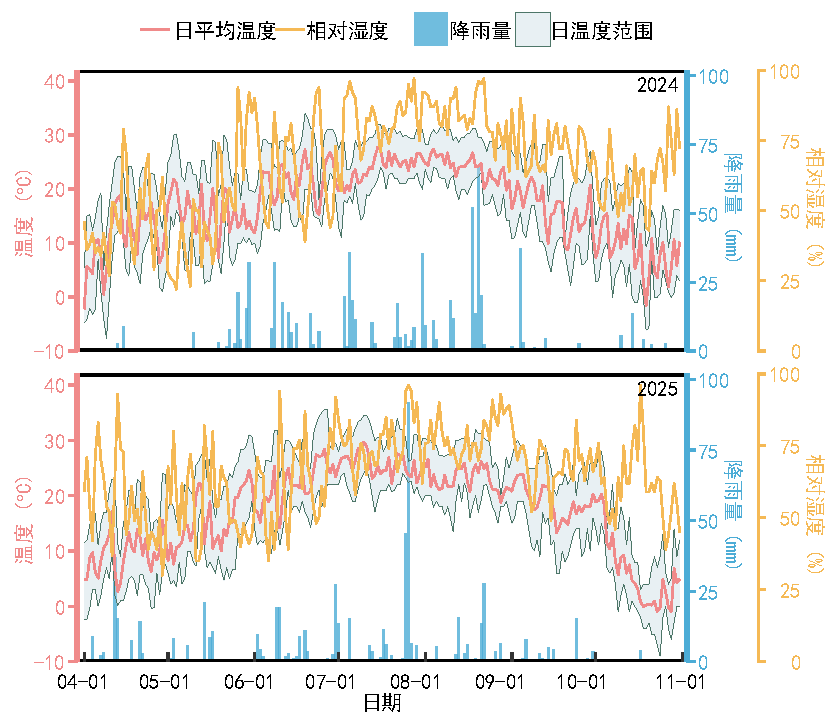
\includegraphics[width=1.0\linewidth]{Figure/qixiang}
		\caption{2024 年和 2025 年试验地大豆全生育期温度、湿度、降雨量变化趋势}
		\label{fig:tianqi}
		\footnotesize 气象数据来源于 Meteostat 开放气象数据平台（https://meteostat.net/）。数据最后访问日期：2026 年 2 月 22 日。
	\end{figure}
	
	\section{试验材料与试验设计}
	
	本章针对引言中提出的三个核心研究问题，系统开展材料准备与试验设计工作。
	
	\subsection{供试材料}
	
	试大豆材料为吉林大学植物科学学院通过美国扁茎与中国扁茎（Glycine max (L.) Merr.）经多年杂交选育而成的后代稳定品系 LFI297。该品系的选择基于以下理由：（1）遗传背景清晰，经过多年选育已达到遗传稳定状态；（2）具有顶生花序簇生、耐密植、分枝角度小以及结荚密集的生物学特征（图~\ref{fig:lf297}），这些特征使其成为研究耐密理想株型的理想材料；（3）适用于大豆株型改良与高光效育种研究，能够为大豆产量突破提供新的种质资源。
	
	\begin{figure}[htb]
		\centering
		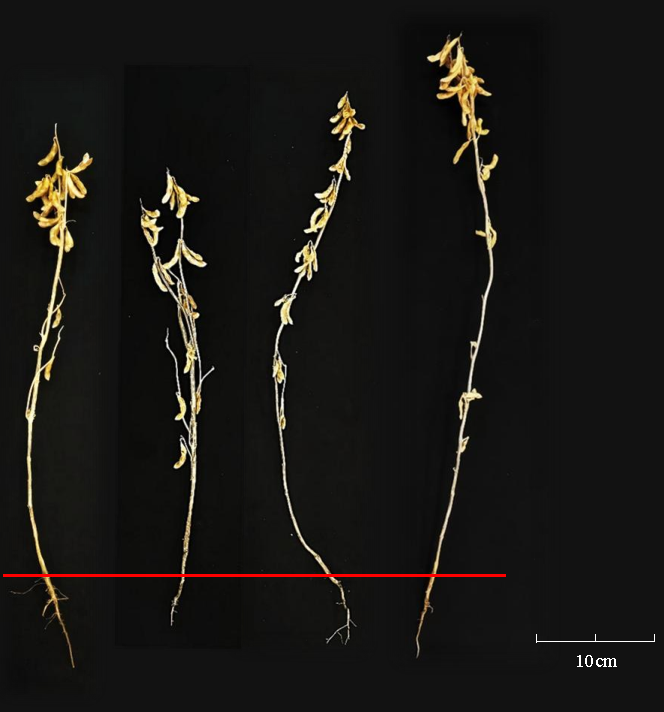
\includegraphics[width=0.5\linewidth]{Figure/plant}
		\caption{2025 年不同种植密度下扁茎大豆后代稳定品系 LFI297 代表性植株形态对比}
		\label{fig:lf297}
		\footnotesize 从左至右依次为：30 万株/hm$^2$、35 万株/hm$^2$、40 万株/hm$^2$、55 万株/hm$^2$
	\end{figure}
		
	\chapter{结果与分析}

	本章系统分析种植密度对扁茎大豆后代稳定品系 LFI297 农艺性状、产量构成、冠层结构及品质的影响，主要包括：(1) 明确 LFI297 产量随密度变化的动态响应规律；(2) 筛选影响单株生产力的关键因子；(3) 评价其在不同密度下的营养品质特征。
	
	\section{种植密度对扁茎大豆后代稳定品系 LFI297 农艺性状及群体产量的影响}
	
	对两年不同密度处理下的各性状分别进行单因素方差分析（One-way ANOVA），设定显著水平 $\alpha = 0.05$ ，并采用 Duncan's 新复极差法对存在显著差异的性状进行多重比较。为探究主要性状随密度变化的定量变化规律，以密度为自变量、各性状为因变量，分别拟合一次线性、对数、二次多项式、指数、幂函数和双曲线模型，根据$R^2$选择最优拟合预测模型（结果均为二次多项式模型）。
	
	\begin{equation}
		\begin{aligned}
			&\textbf{线性模型:} \quad y = a + bx \\
			&\textbf{对数模型:} \quad y = a + b \ln(x) \\
			&\textbf{二次多项式模型:} \quad y = ax^2 + bx + c \\
			&\textbf{指数模型:} \quad y = a e^{bx}\\
			&\textbf{幂函数模型:} \quad y = a x^b \\
			&\textbf{双曲线模型:} \quad y = a + \frac{b}{x}
		\end{aligned}
	\end{equation}
	
	其中，$y$ 为因变量（产量、株高、单株荚数等）；$x$ 为自变量（种植密度）；$a, b, c$ 为待定系数。	
	

	\begin{sidewaystable}[htbp]
		\centering
		\caption{2024 年不同种植密度下扁茎大豆后代稳定品系 LFI297 的农艺性状统计分析}
		\label{tab:agri2024}
		\footnotesize % 因为变成了横排，空间变大，可以使用稍大一点的字号
		\setlength{\tabcolsep}{4pt} % 列间距也可以适当放宽，看起来不那么拥挤
		\begin{tikzpicture}[overlay, remember picture]
		\end{tikzpicture}
		\begin{tabular}{lccccccccccccccccc}
			\toprule
			\makecell[l]{密度\\(万株/\\hm$^2$)} & \makecell{产量\\(kg/\\hm$^2$)} & \makecell{株高\\(cm)} & \makecell{分枝\\角度\\($^\circ$)} & \makecell{节数\\(节)} & \makecell{一级\\分枝\\数(个)} & \makecell{单株\\荚数\\(个)} & \makecell{顶生\\花序\\长度\\(cm)} & \makecell{顶生\\花序\\荚数\\(个)} & \makecell{顶生\\花序\\粒数\\(粒)} & \makecell{顶生\\花序\\百粒\\重(g)} & \makecell{顶生\\花序\\粒重\\(g)} & \makecell{单株\\粒数\\(粒)} & \makecell{单株\\粒重\\(g)} & \makecell{百粒\\重\\(g)} & \makecell{顶端\\贡献\\率(\%)} & \makecell{叶绿素相对含量\\(SPAD)} & \makecell{氮含\\量\\(mg/g)} \\
			\midrule
			24 & 3757.29 b & 58.42 a & 20.99 a & 9.86 a & 4.80 a & 45.74 a & 13.31 b & 6.52 a & 13.07 a & 19.36 a & 2.35 a & 92.16 a & 15.66 a & 17.15 a & 21.22 a & 55.20 a & 18.06 a \\
			30 & 4876.00 a & 61.92 a & 17.89 a & 10.17 a & 5.87 a & 51.27 a & 18.56 a & 9.02 a & 17.72 a & 19.06 a & 3.16 a & 102.20 a & 16.25 a & 17.66 a & 24.36 a & 53.41 a & 17.44 a \\
			34 & 5067.18 a & 63.37 a & 16.50 a & 9.59 a & 4.88 a & 54.35 a & 17.70 a & 6.12 a & 13.25 a & 15.87 b & 2.90 a & 108.34 a & 14.90 a & 16.08 a & 26.90 a & 51.51 a & 16.17 a \\
			\hdashline
			参数 & & & & & & & & & & & & & & & & & \\
		    平均值 & 4504.28 & 60.97 & 18.71 & 9.91 & 5.22 & 49.97 & 16.38 & 7.36 & 14.86 & 18.38 & 2.79 & 99.97 & 15.69 & 17.08 & 23.82 & 53.90 & 17.52 \\
			标准差 & 737.03 & 4.67 & 5.76 & 0.69 & 1.19 & 9.28 & 2.90 & 2.19 & 4.15 & 1.85 & 0.65 & 18.94 & 1.55 & 1.38 & 4.80 & 6.80 & 1.21 \\
			变异系数 & 16.36\% & 7.66\% & 30.80\% & 6.95\% & 22.80\% & 18.58\% & 17.70\% & 29.78\% & 27.95\% & 10.06\% & 23.13\% & 18.95\% & 9.90\% & 8.07\% & 20.17\% & 12.62\% & 6.89\% \\
			F & 6.30* & 0.71 & 0.33 & 0.35 & 0.64 & 0.48 & 9.01* & 1.66 & 1.21 & 6.01* & 1.35 & 0.39 & 0.37 & 0.74 & 0.83 & 0.09 & 0.90 \\
			P & 0.043 & 0.536 & 0.731 & 0.720 & 0.567 & 0.645 & 0.022 & 0.279 & 0.373 & 0.047 & 0.339 & 0.697 & 0.707 & 0.521 & 0.489 & 0.919 & 0.476 \\
			\bottomrule
			\multicolumn{18}{l}{不同小写字母表示不同处理间差异显著($P < 0.05$)。F 表示方差分析，P 表示方差分析的显著性检验。*表示 $P < 0.05$，**表示 $P < 0.01$，***表示 $P < 0.001$。}
		\end{tabular}
		\vspace{0.5cm} % 两个表之间的间距
		% F表示方差分析，P表示显著性检验。*表示 $P < 0.05$，**表示 $P < 0.01$，***表示 $P < 0.001$。
	
		
		\centering
		\caption{2025 年不同种植密度下扁茎大豆后代稳定品系 LFI297 的农艺性状统计分析}
		\label{tab:agri2025}
		\footnotesize
		\setlength{\tabcolsep}{3.5pt}
		\begin{tabular}{lcccccccccccccccccc}
			\toprule
			\makecell[l]{密度\\(万株/\\hm$^2$)} & \makecell{产量\\(kg/\\hm$^2$)} & \makecell{株高\\(cm)} & \makecell{分枝\\角度\\($^\circ$)} & \makecell{节数\\(节)} & \makecell{一级\\分枝\\数(个)} & \makecell{单株\\荚数\\(个)} & \makecell{顶生\\花序\\长度\\(cm)} & \makecell{顶生\\花序\\节(节)} & \makecell{顶生\\花序\\荚数\\(个)} & \makecell{顶生\\花序\\粒数\\(粒)} & \makecell{顶生\\花序\\百粒\\重(g)} & \makecell{顶生\\花序\\粒重\\(g)} & \makecell{单株\\粒数\\(粒)} & \makecell{单株\\粒重\\(g)} & \makecell{百粒\\重\\(g)} & \makecell{顶端\\贡献\\率(\%)} & \makecell{蛋白\\质\\(\%)} & \makecell{油分\\(\%)} \\
			\midrule
			30 & 3322.23 b & 70.15 a & 28.40 a & 11.33 a & 4.42 a & 35.50 a & 18.07 b & 7.97 a & 8.06 a & 15.24 a & 19.58 a & 2.71 a & 59.87 a & 11.07 a & 19.58 a & 31.38 b & 36.71 a & 19.58 a \\
			35 & 4156.42 a & 68.16 a & 29.66 a & 10.74 a & 3.92 b & 34.03 a & 18.03 b & 6.79 a & 6.37 a & 12.54 a & 19.81 a & 2.36 a & 61.61 a & 11.88 a & 19.72 a & 27.26 b & 36.78 a & 19.77 a \\
			40 & 3647.14 b & 69.55 a & 25.73 a & 10.98 a & 3.90 b & 30.20 a & 17.13 b & 7.29 a & 8.00 a & 14.88 a & 20.41 a & 2.71 a & 50.22 b & 9.12 b & 19.65 a & 35.69 b & 37.09 a & 19.66 a \\
			55 & 3578.43 b & 72.58 a & 21.91 a & 10.78 a & 2.87 c & 25.91 a & 20.57 a & 7.99 a & 7.80 a & 13.86 a & 19.91 a & 2.58 a & 35.75 c & 6.51 c & 19.68 a & 50.56 a & 37.72 a & 19.32 a \\
			\hdashline
			参数\\
			平均值 & 3676.06 & 70.11 & 26.43 & 10.96 & 3.78 & 31.41 & 18.45 & 7.51 & 7.56 & 14.13 & 19.93 & 2.59 & 51.86 & 9.64 & 19.66 & 36.22 & 37.08 & 19.58 \\
			标准差 & 347.05 & 2.43 & 4.04 & 0.59 & 0.61 & 4.47 & 1.45 & 0.68 & 0.95 & 2.18 & 0.58 & 0.33 & 11.05 & 2.24 & 0.35 & 10.01 & 0.67 & 0.33 \\
			变异系数 & 9.44\% & 3.46\% & 15.31\% & 5.39\% & 16.23\% & 14.22\% & 7.85\% & 9.04\% & 12.57\% & 15.41\% & 2.89\% & 12.85\% & 21.31\% & 23.18\% & 1.77\% & 27.63\% & 1.80\% & 1.69\% \\
			F & 8.84* & 1.31 & 2.14 & 0.29 & 34.52** & 5.04 & 11.04* & 2.20 & 2.03 & 0.48 & 0.62 & 0.34 & 94.51*** & 67.62*** & 0.04 & 10.09* & 0.91 & 0.53 \\
			P & 0.031 & 0.387 & 0.237 & 0.833 & 0.003 & 0.076 & 0.021 & 0.230 & 0.252 & 0.713 & 0.636 & 0.798 & 0.000 & 0.001 & 0.990 & 0.025 & 0.511 & 0.686 \\
			\bottomrule
			\multicolumn{19}{l}{\footnotesize 不同小写字母表示不同处理间差异显著($P < 0.05$)。F 表示方差分析，P 表示方差分析的显著性检验。*表示 $P < 0.05$，**表示 $P < 0.01$，***表示 $P < 0.001$。}
		\end{tabular}
	\end{sidewaystable}
	
	\begin{figure}[htbp]
		\centering
		\begin{overpic}[width=0.24\textwidth]{Figure/2024/bar/SY}
			\put(3, 93){\textbf{A}} % 现在这个坐标就是相对于图片的百分比了，正好是左上角
		\end{overpic}
		  	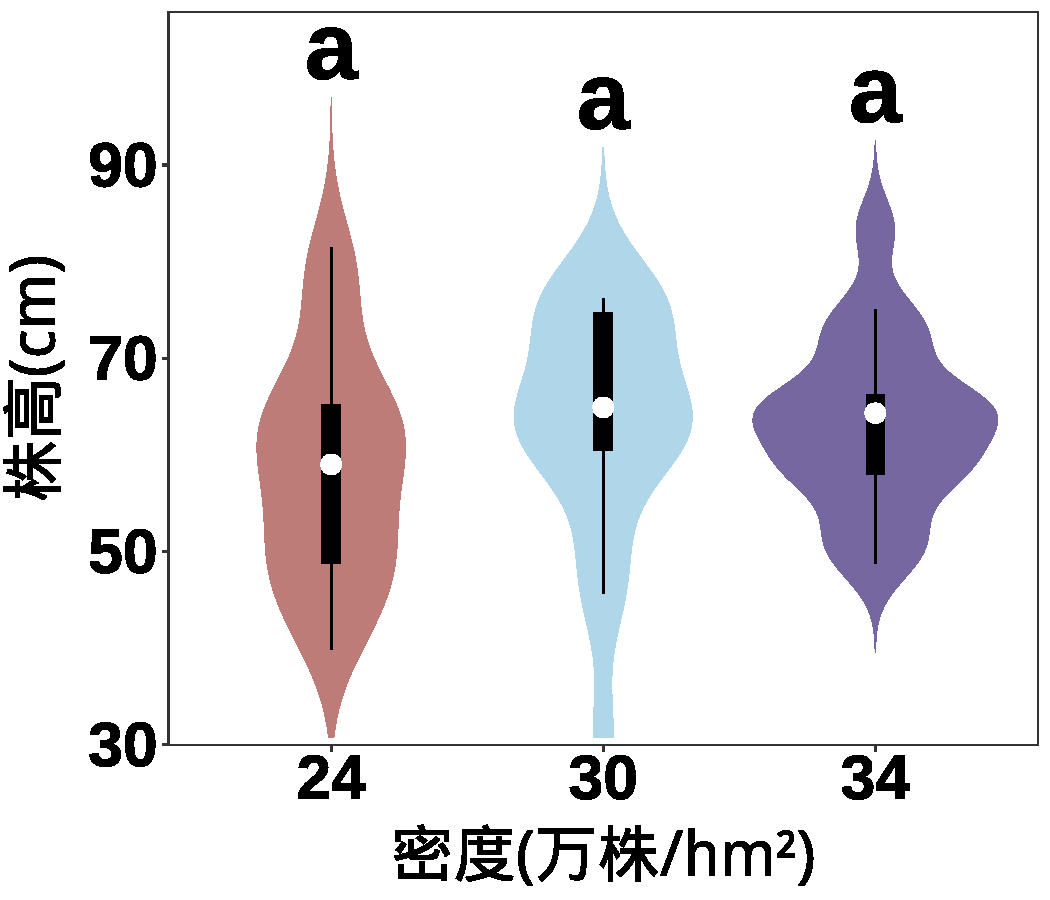
\includegraphics[width=0.24\linewidth]{Figure/2024/bar/PH}
			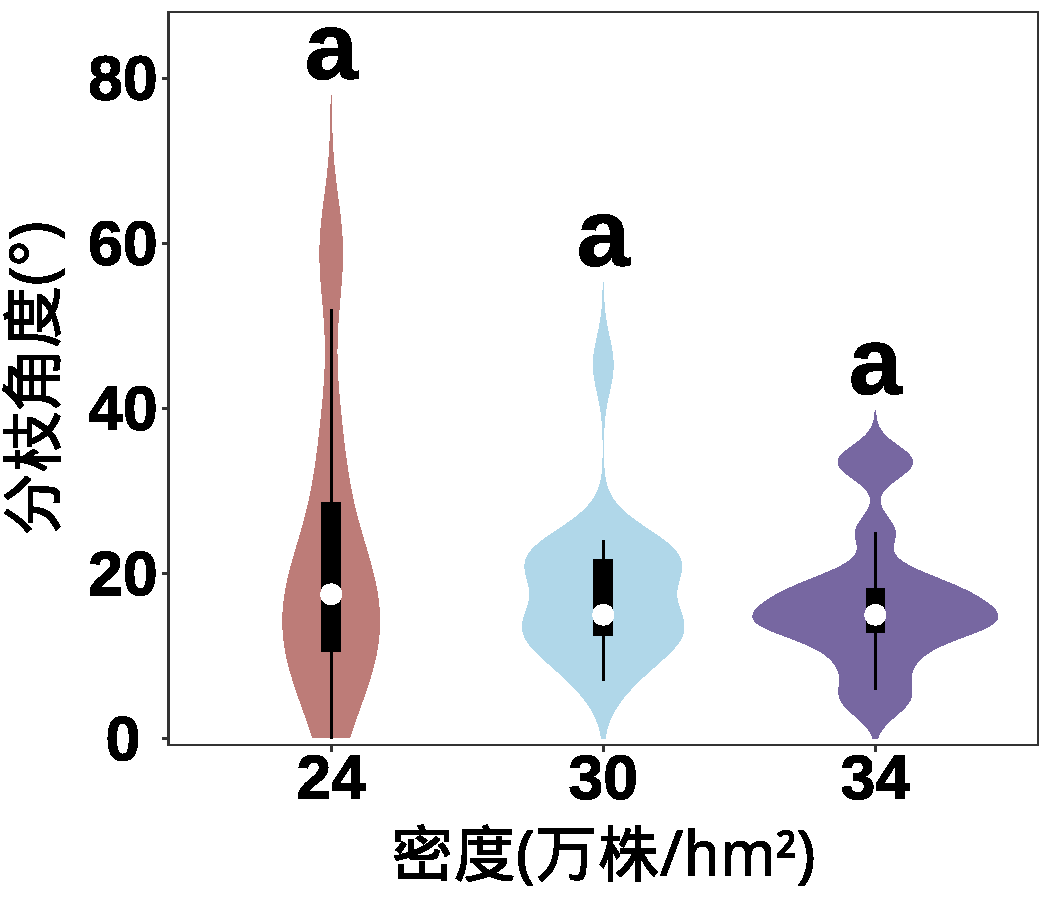
\includegraphics[width=0.24\linewidth]{Figure/2024/bar/BA}
			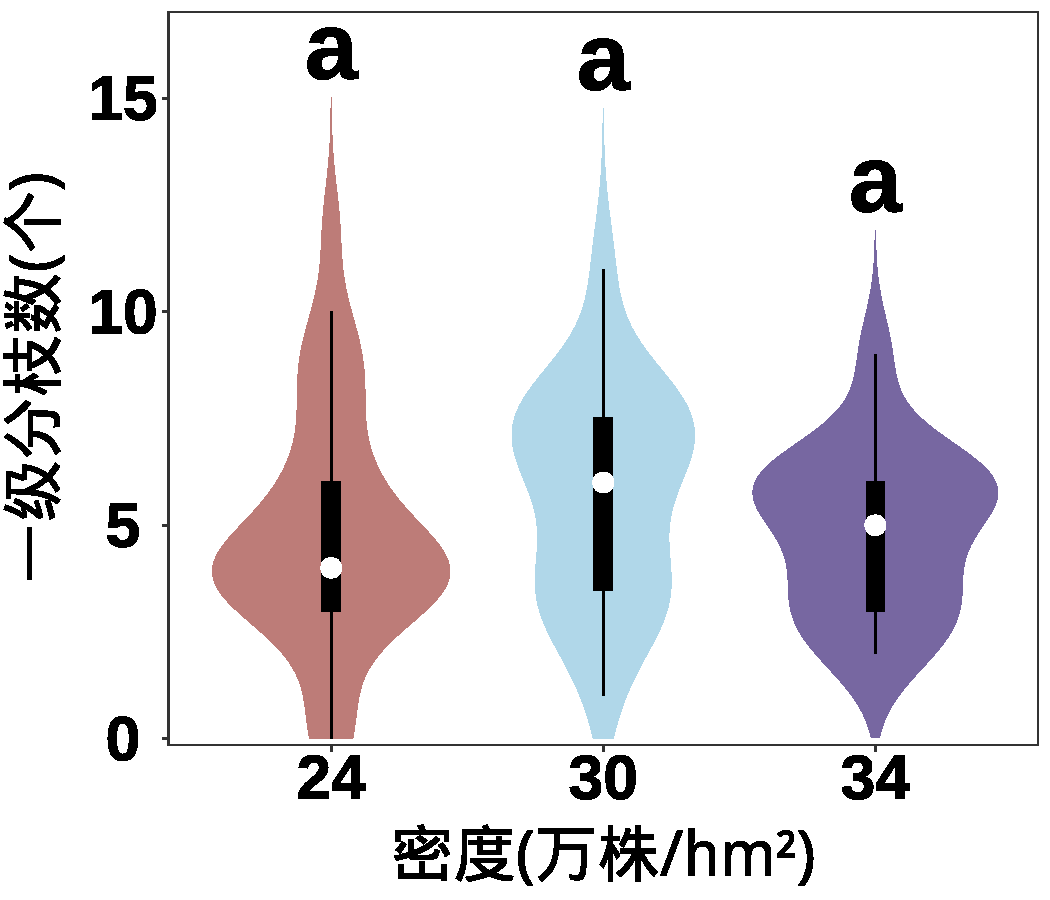
\includegraphics[width=0.24\linewidth]{Figure/2024/bar/NPB}
			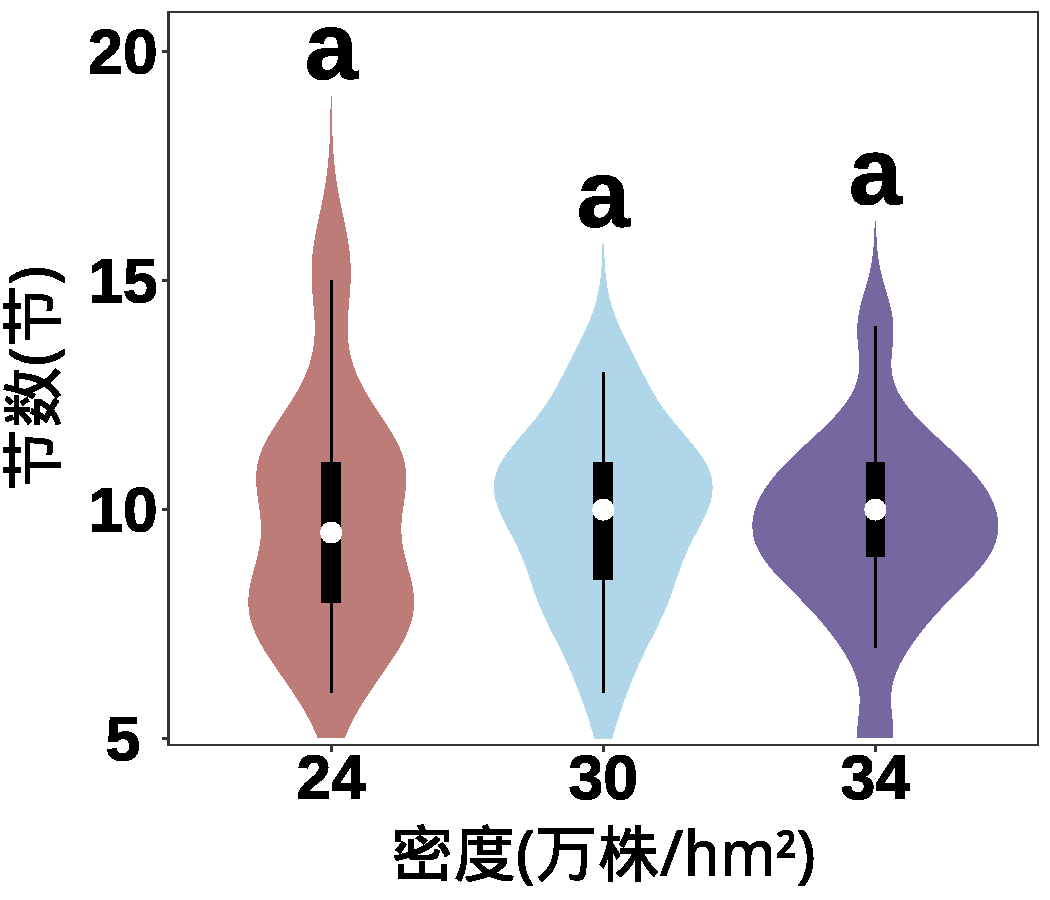
\includegraphics[width=0.24\linewidth]{Figure/2024/bar/MSN}
			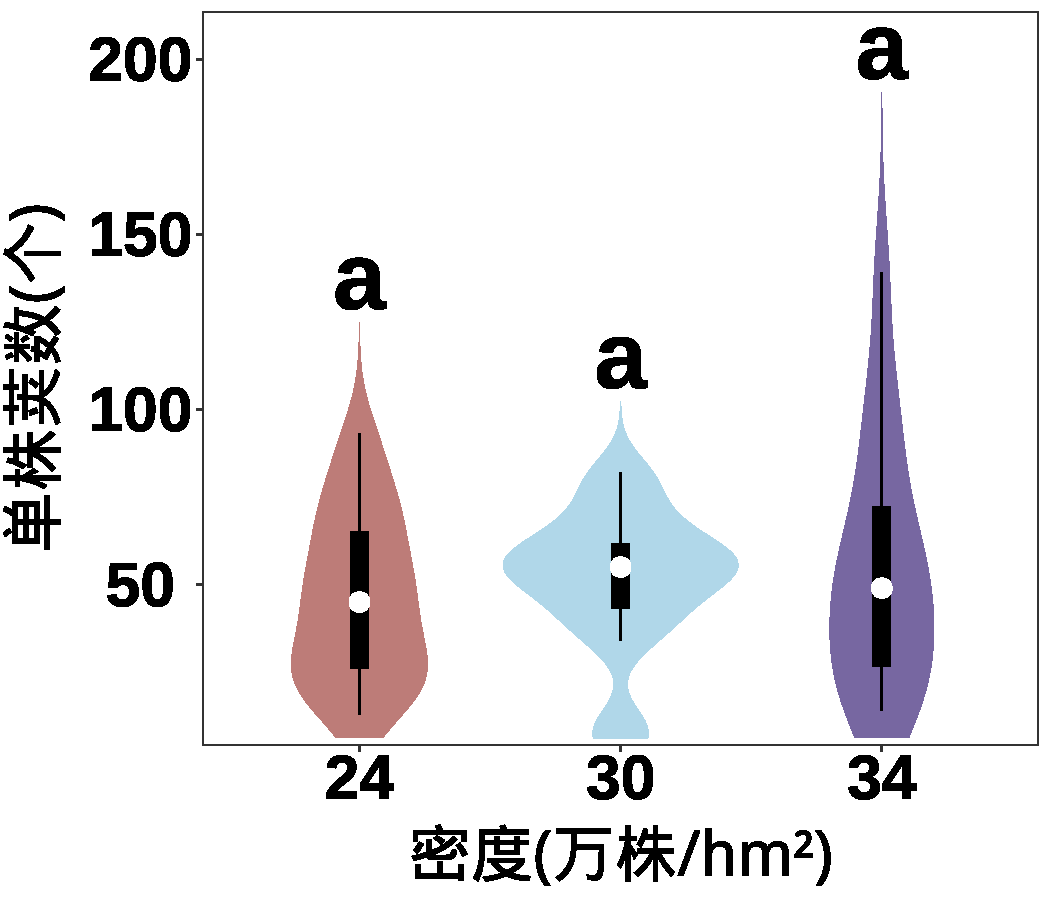
\includegraphics[width=0.24\linewidth]{Figure/2024/bar/PPP}
			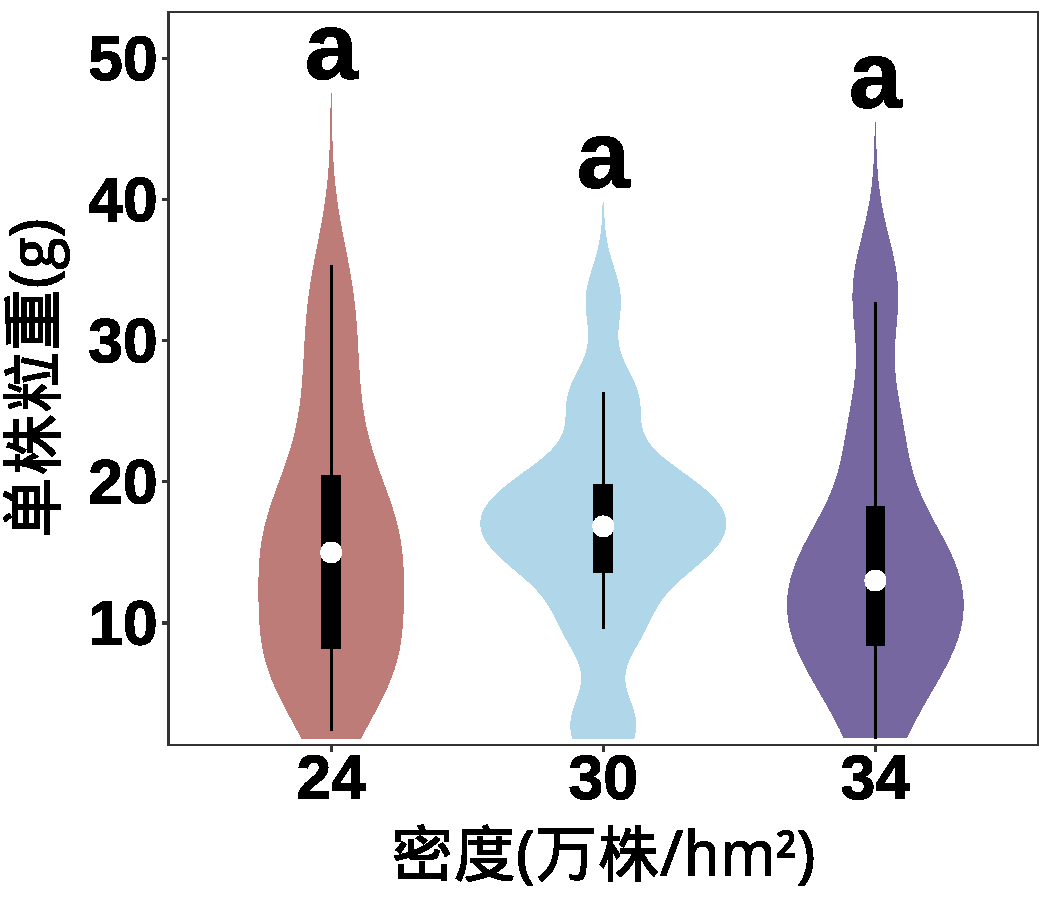
\includegraphics[width=0.24\linewidth]{Figure/2024/bar/SYPP}
			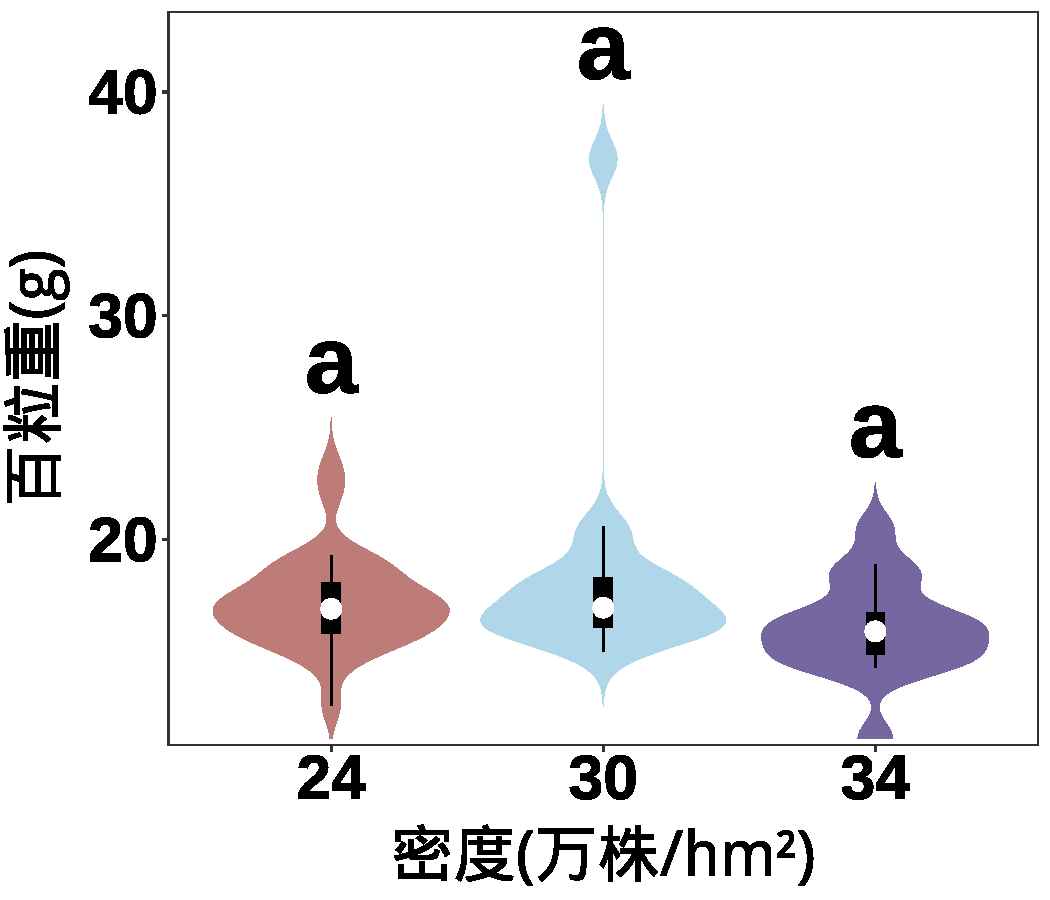
\includegraphics[width=0.24\linewidth]{Figure/2024/bar/HSW}
			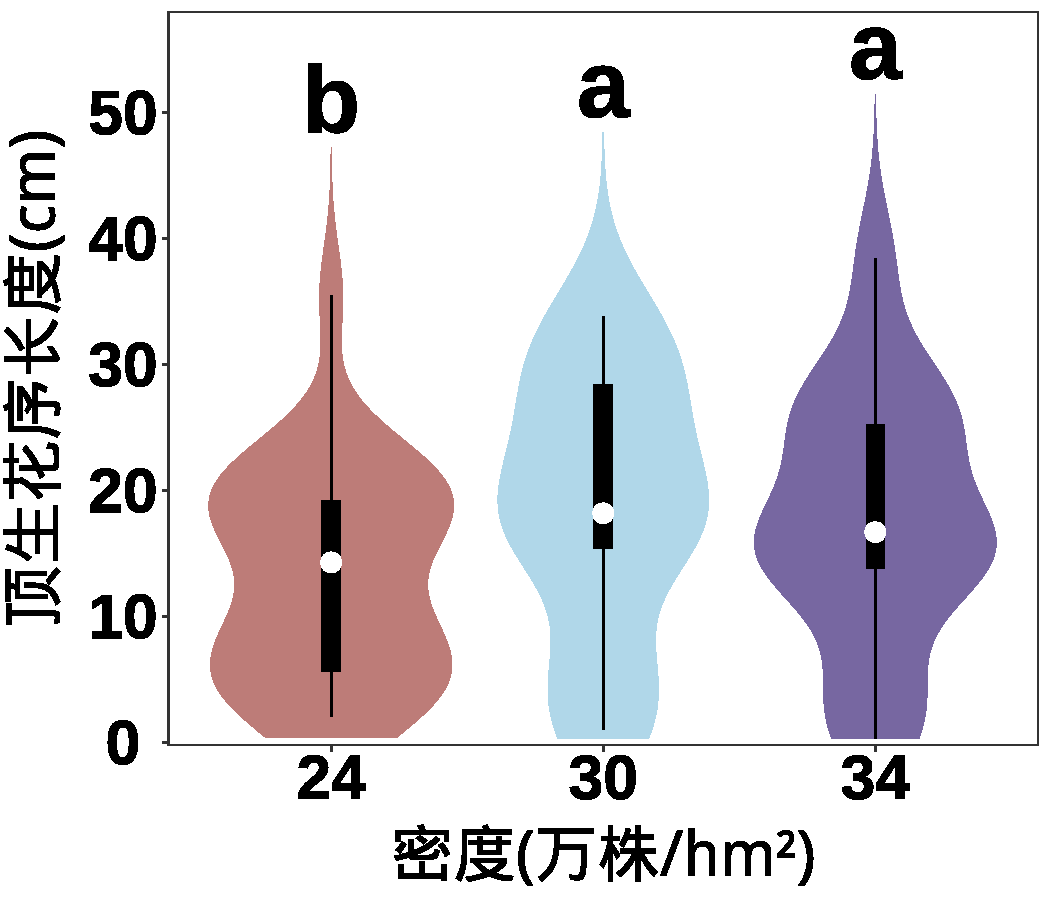
\includegraphics[width=0.24\linewidth]{Figure/2024/bar/TRL}
			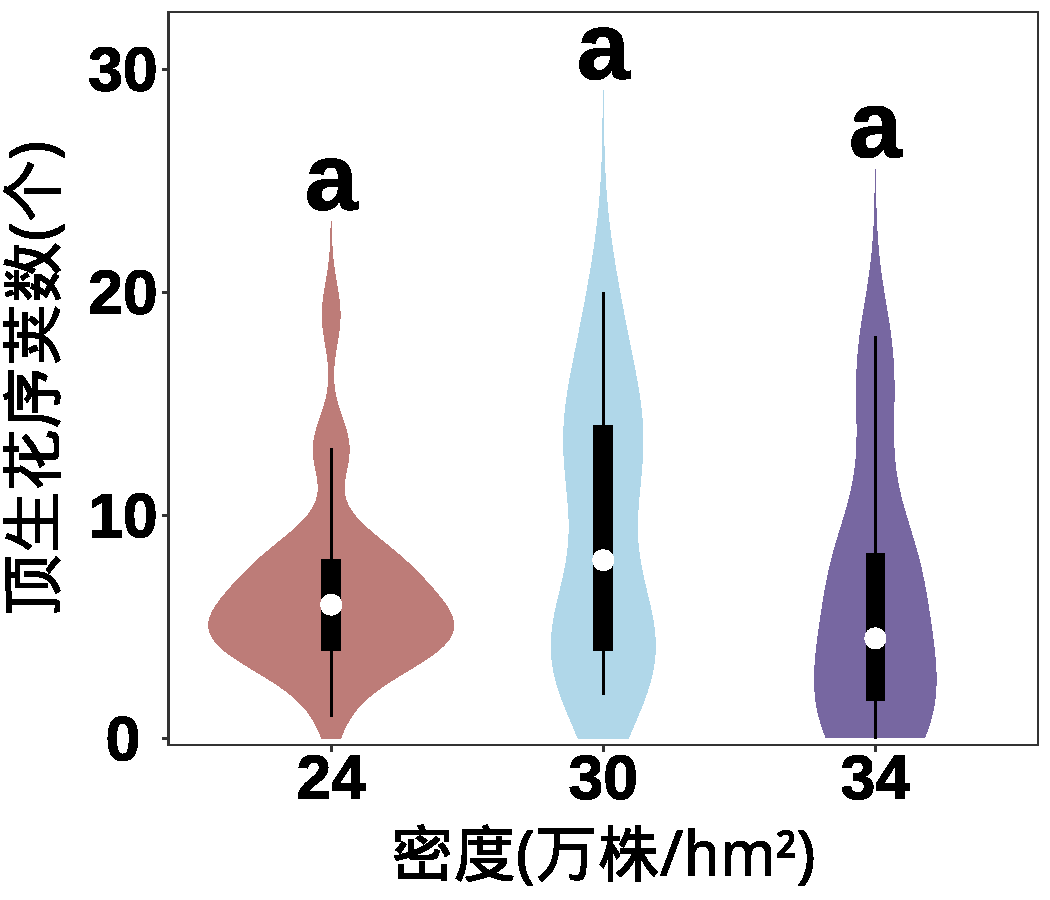
\includegraphics[width=0.24\linewidth]{Figure/2024/bar/PTR}
			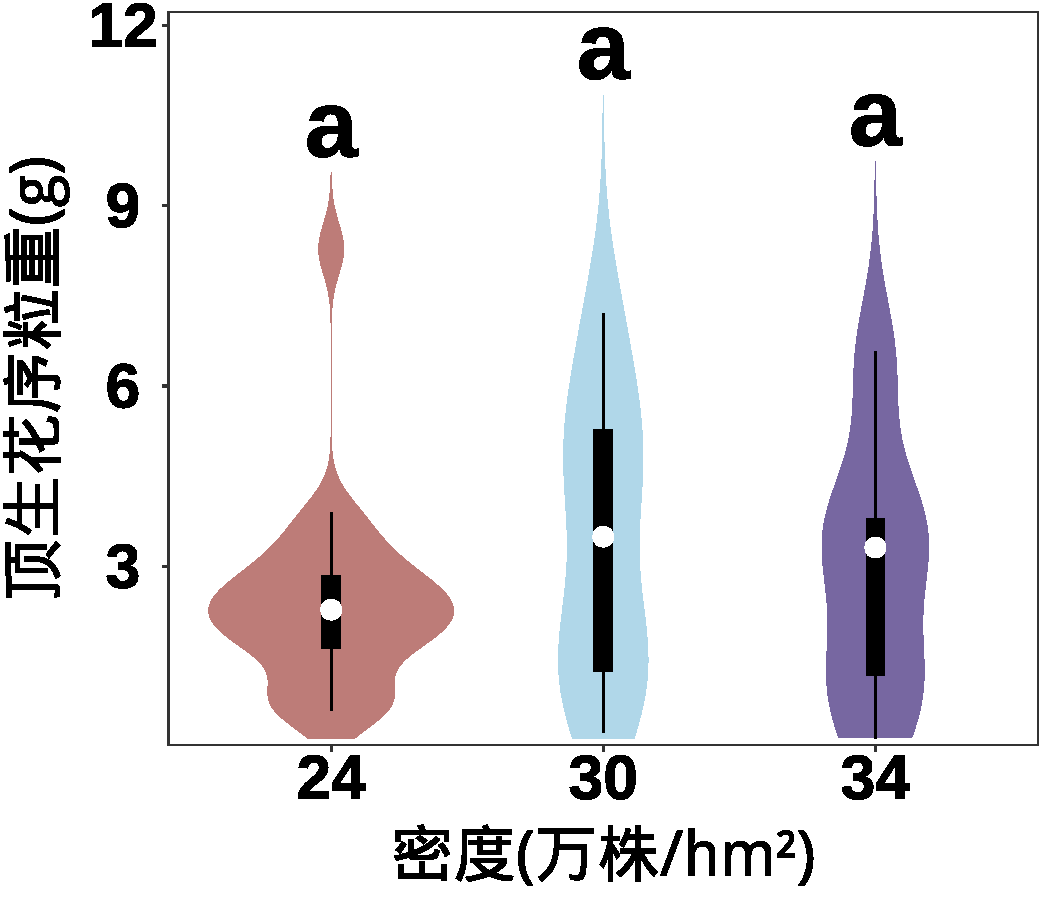
\includegraphics[width=0.24\linewidth]{Figure/2024/bar/TRW}
			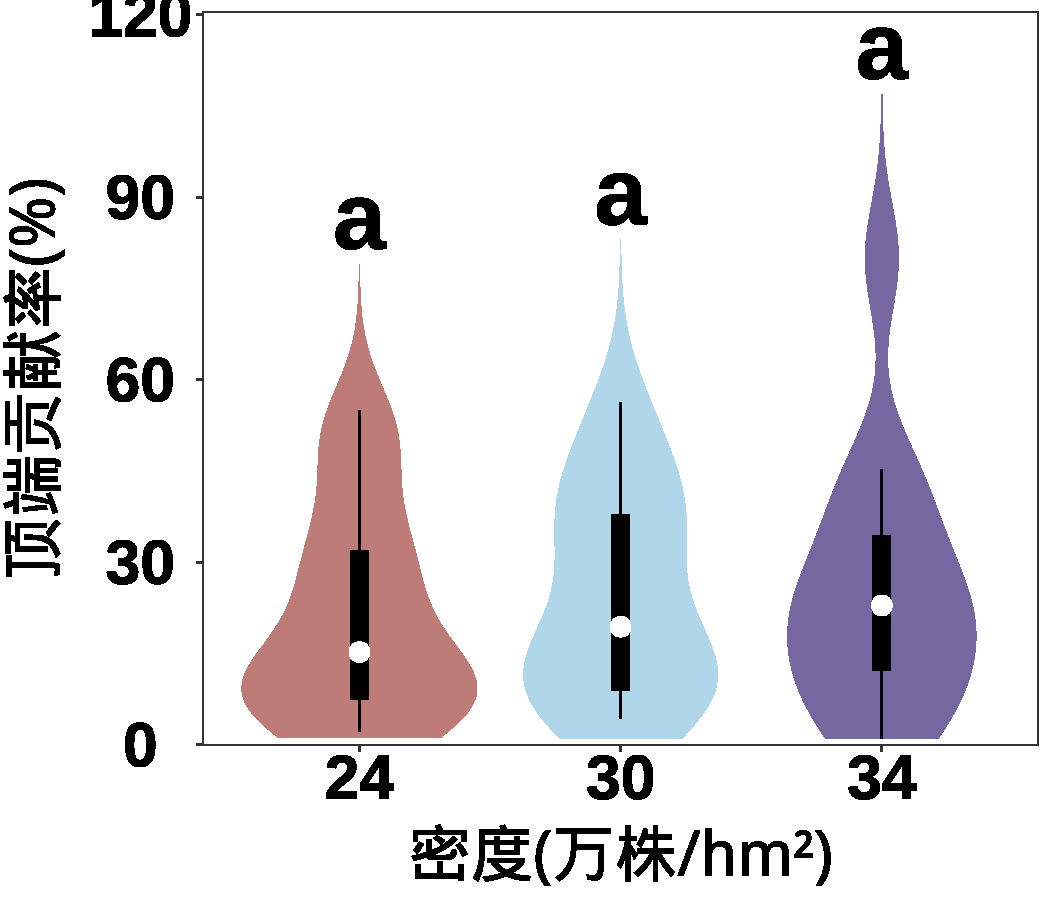
\includegraphics[width=0.24\linewidth]{Figure/2024/bar/CTRY}\vspace{0.5cm}

		\begin{overpic}[width=0.24\textwidth]{Figure/2025/bar/SY}
			\put(3, 93){\textbf{B}}
		\end{overpic}
		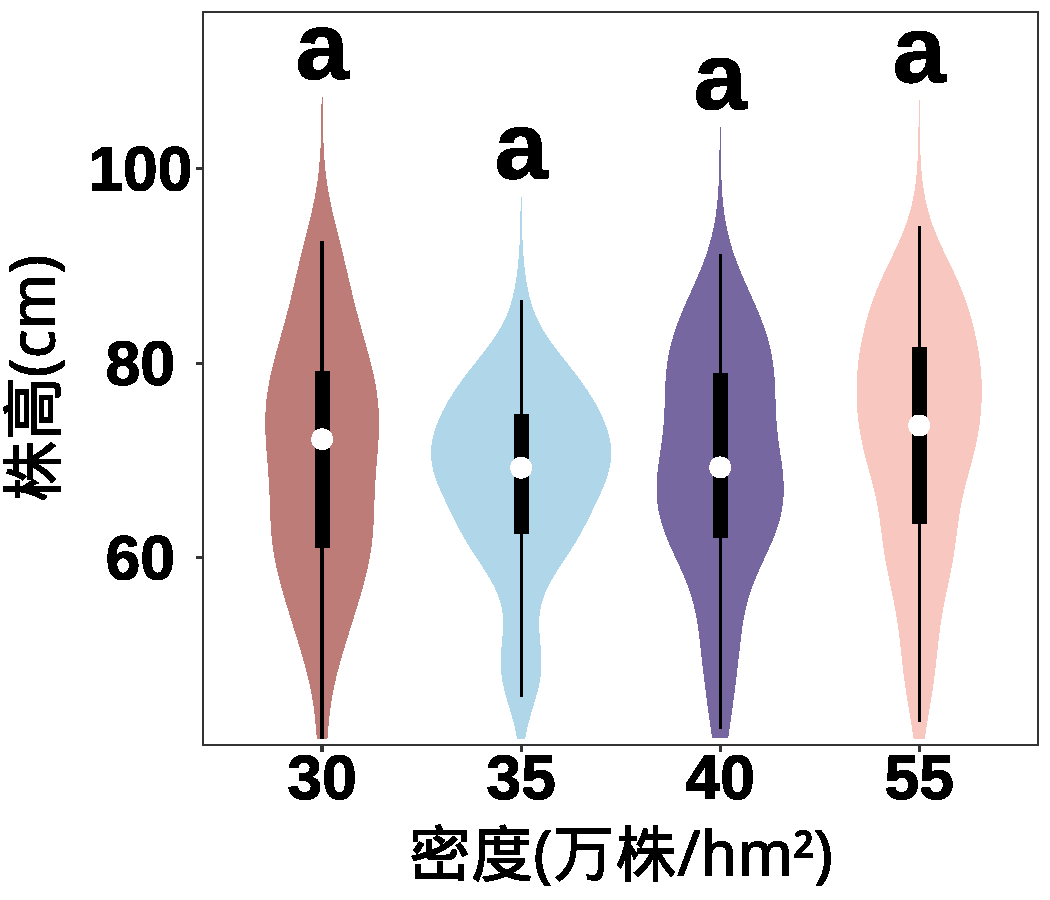
\includegraphics[width=0.24\linewidth]{Figure/2025/bar/PH}
		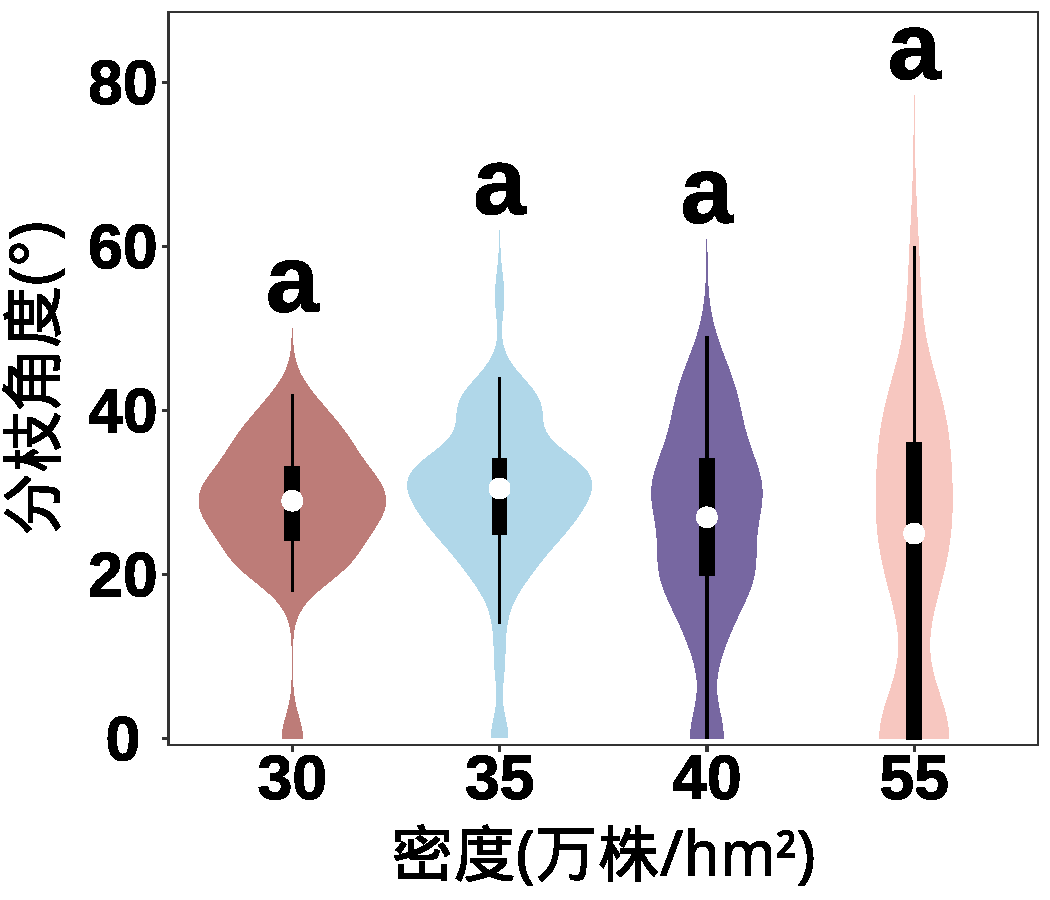
\includegraphics[width=0.24\linewidth]{Figure/2025/bar/BA}
		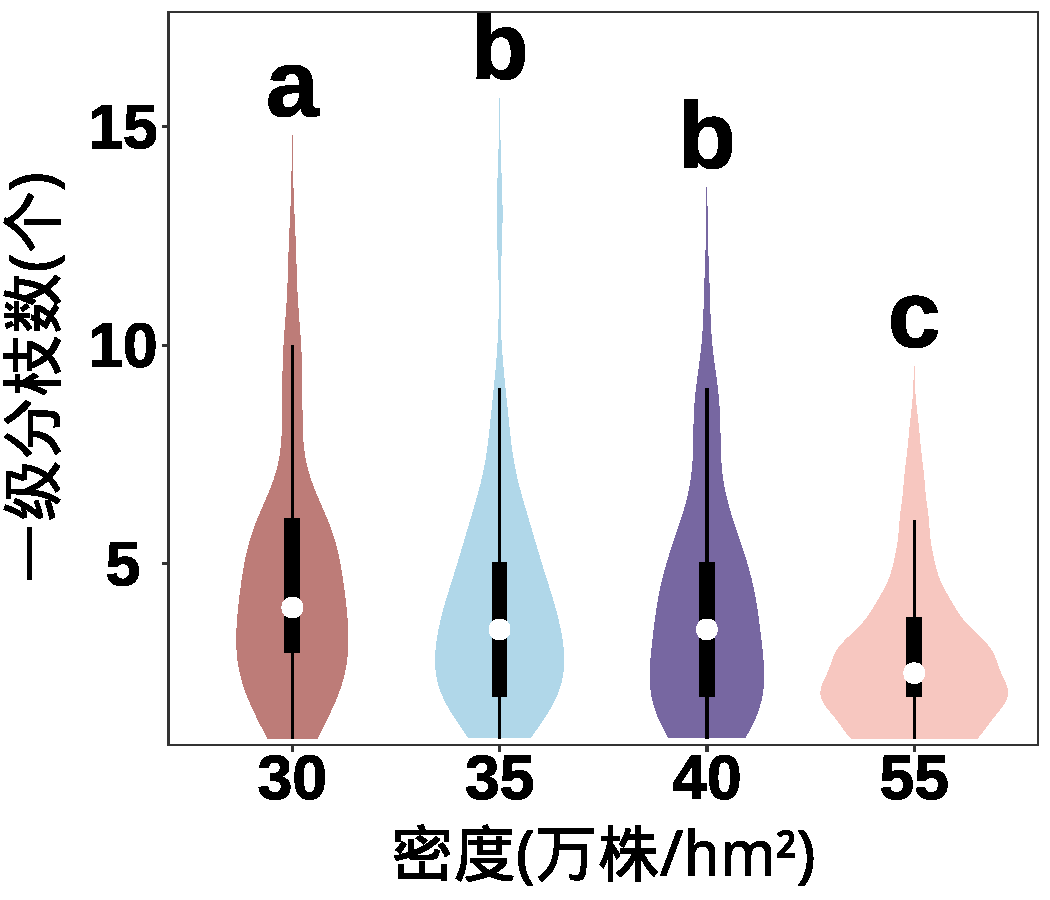
\includegraphics[width=0.24\linewidth]{Figure/2025/bar/NPB}
		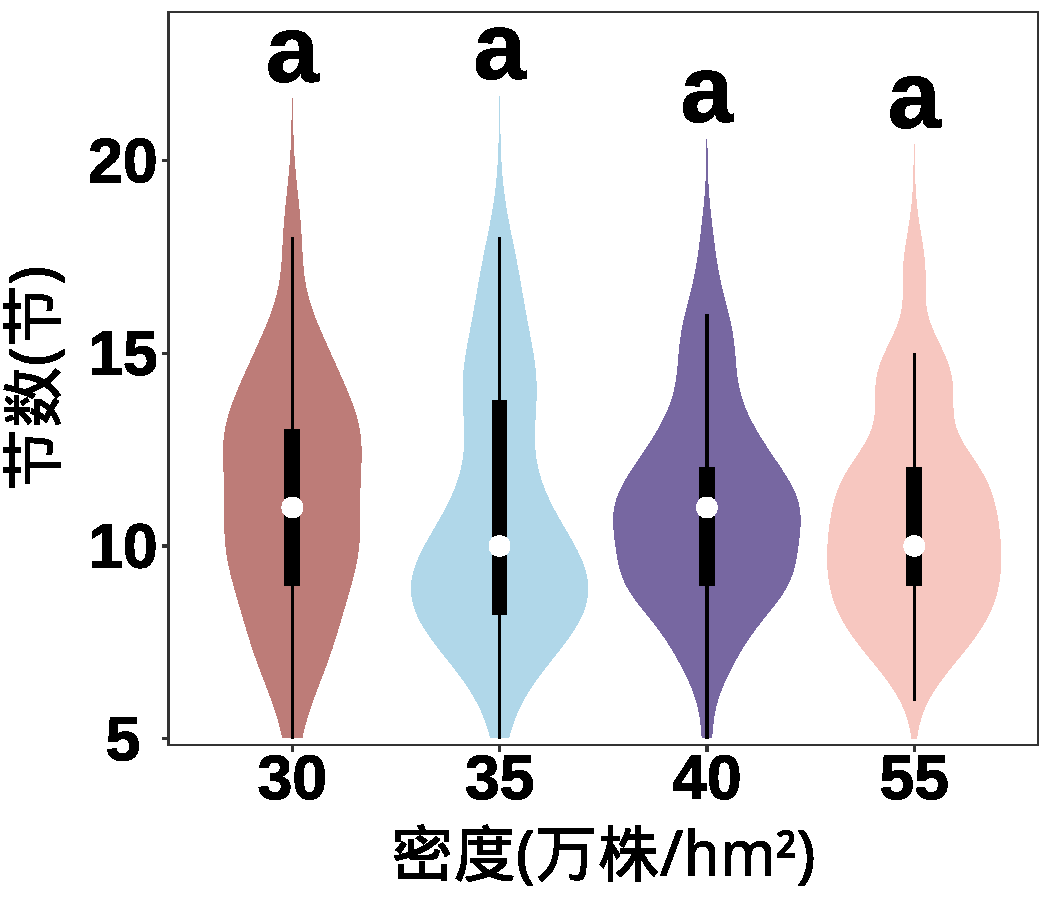
\includegraphics[width=0.24\linewidth]{Figure/2025/bar/MSN}
		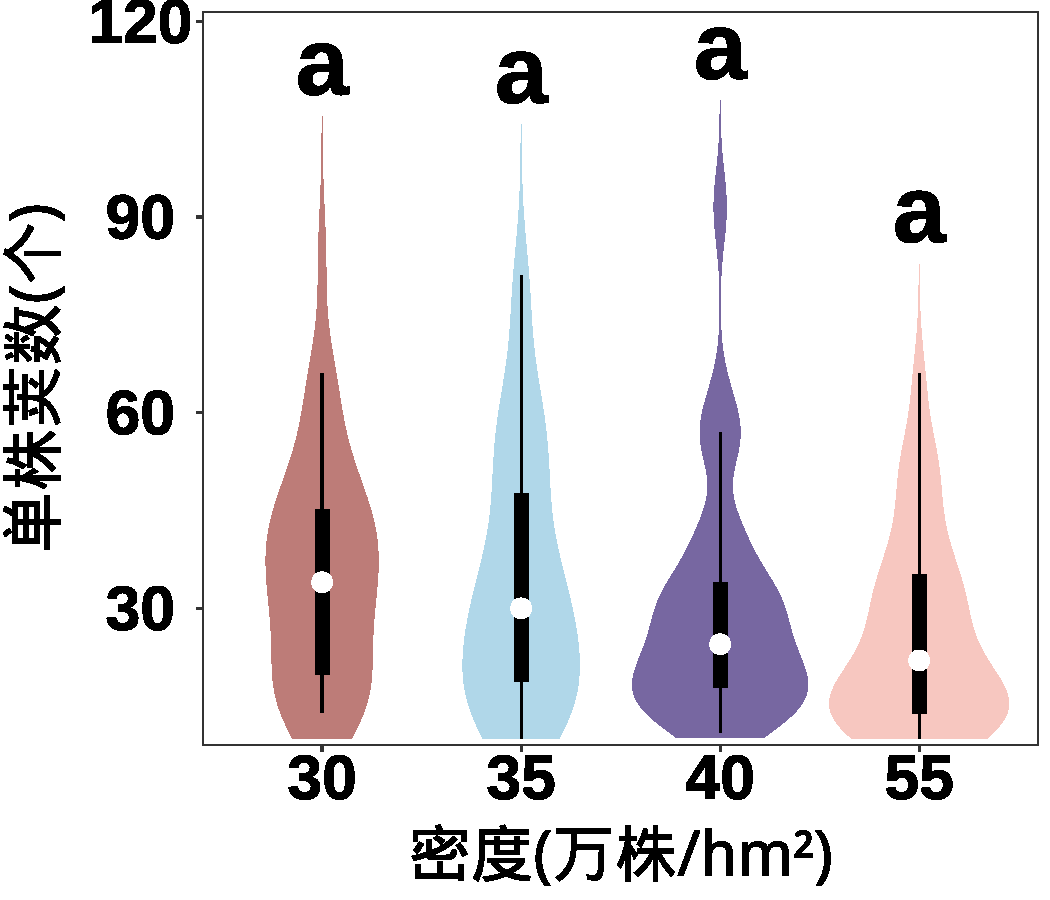
\includegraphics[width=0.24\linewidth]{Figure/2025/bar/PPP}
		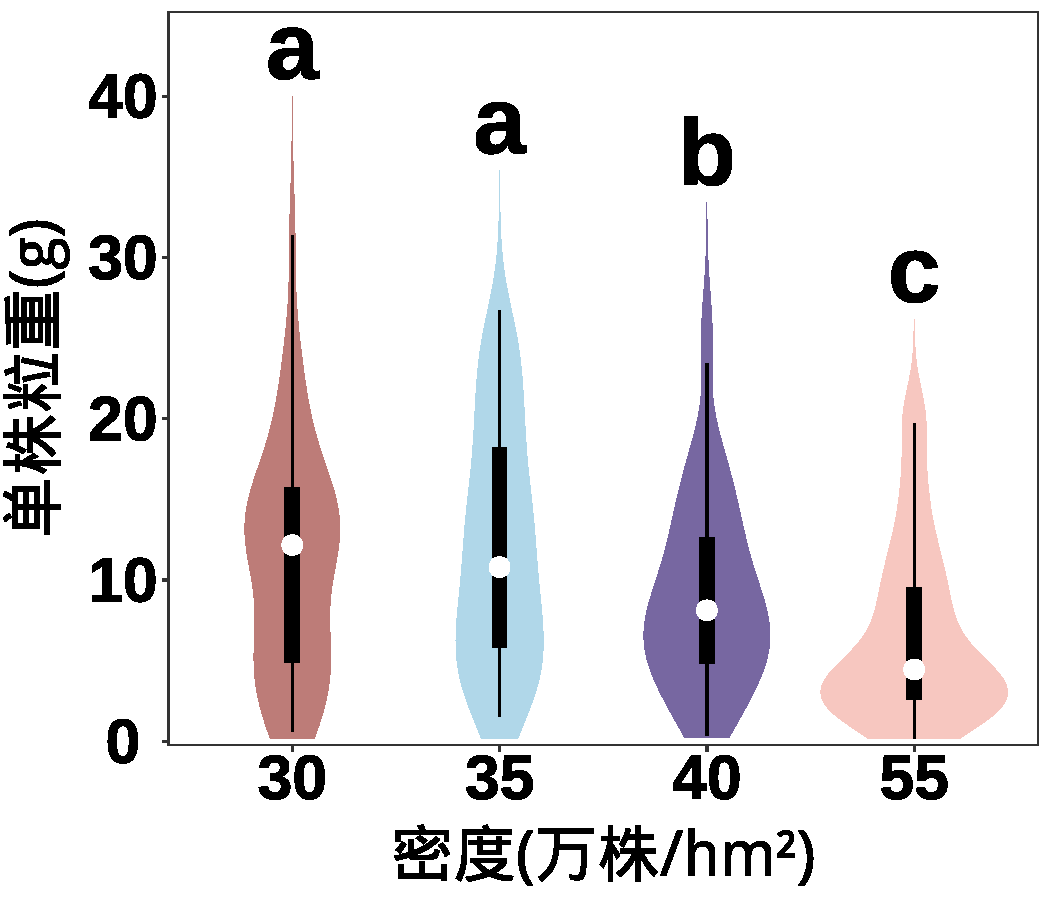
\includegraphics[width=0.24\linewidth]{Figure/2025/bar/SYPP}
		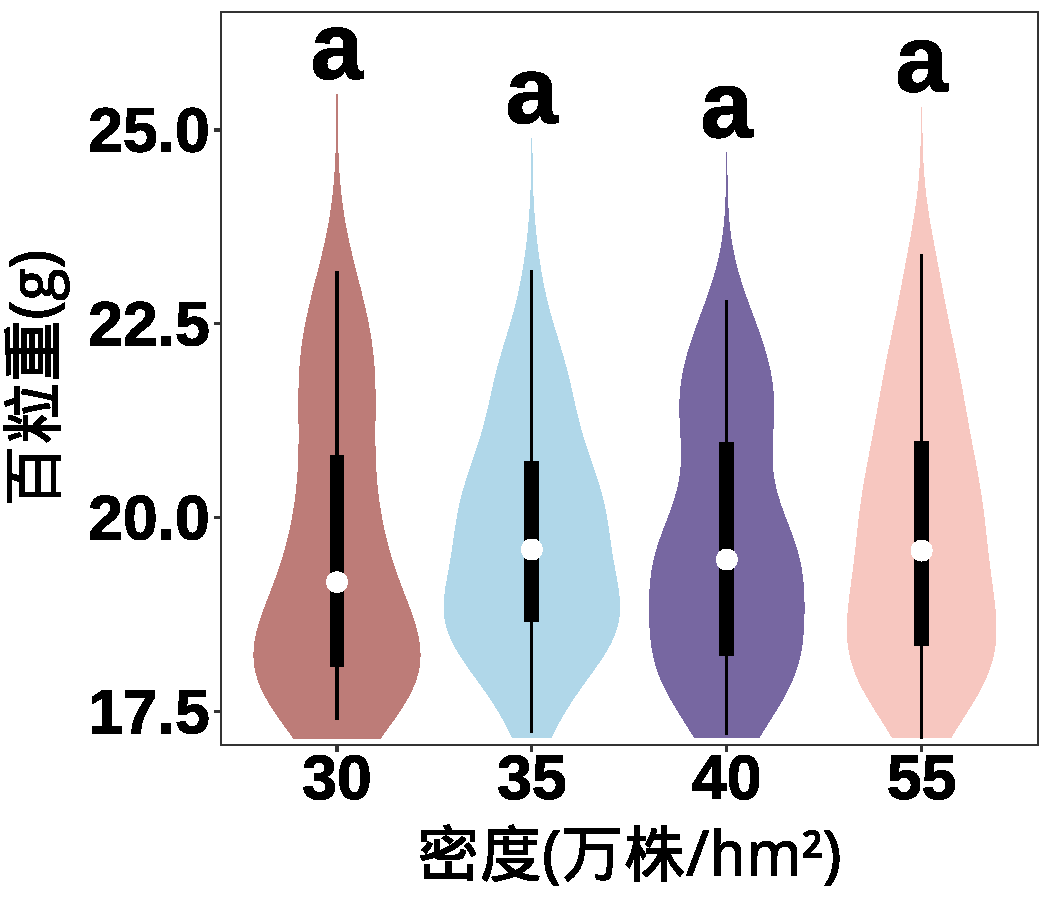
\includegraphics[width=0.24\linewidth]{Figure/2025/bar/HSW}
		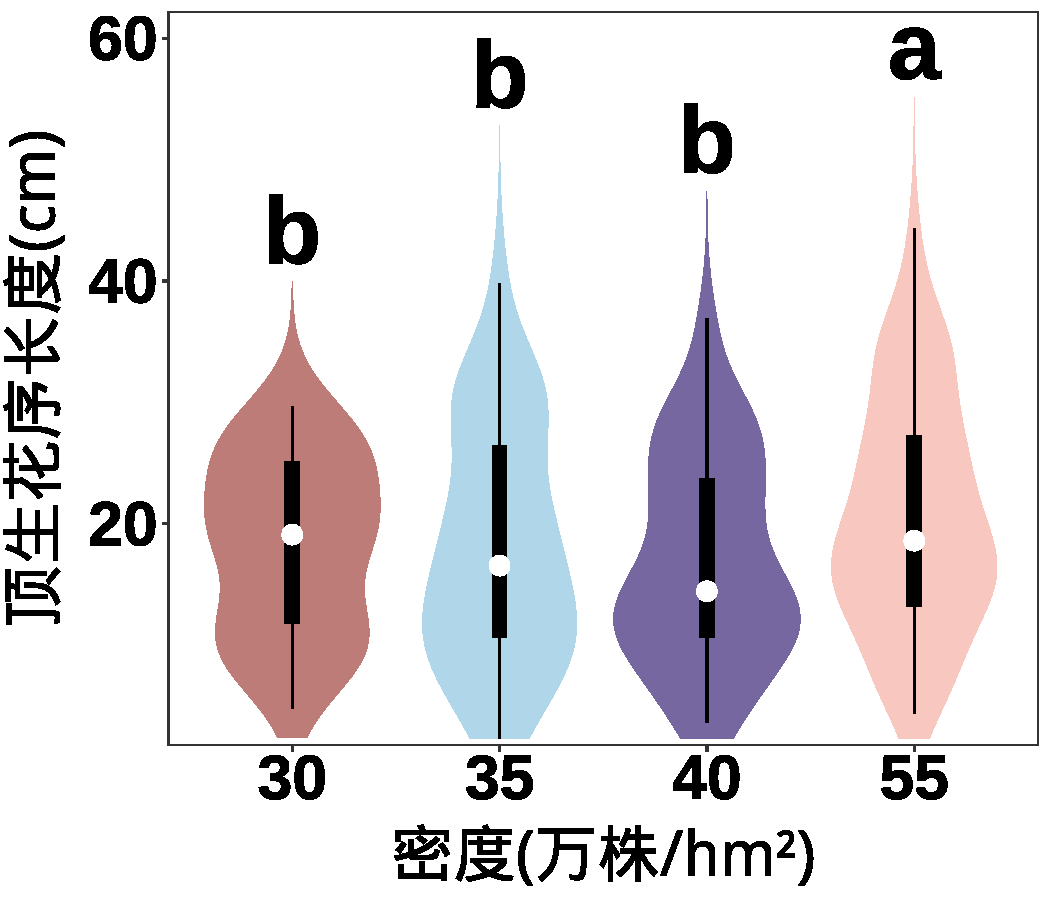
\includegraphics[width=0.24\linewidth]{Figure/2025/bar/TRL}
		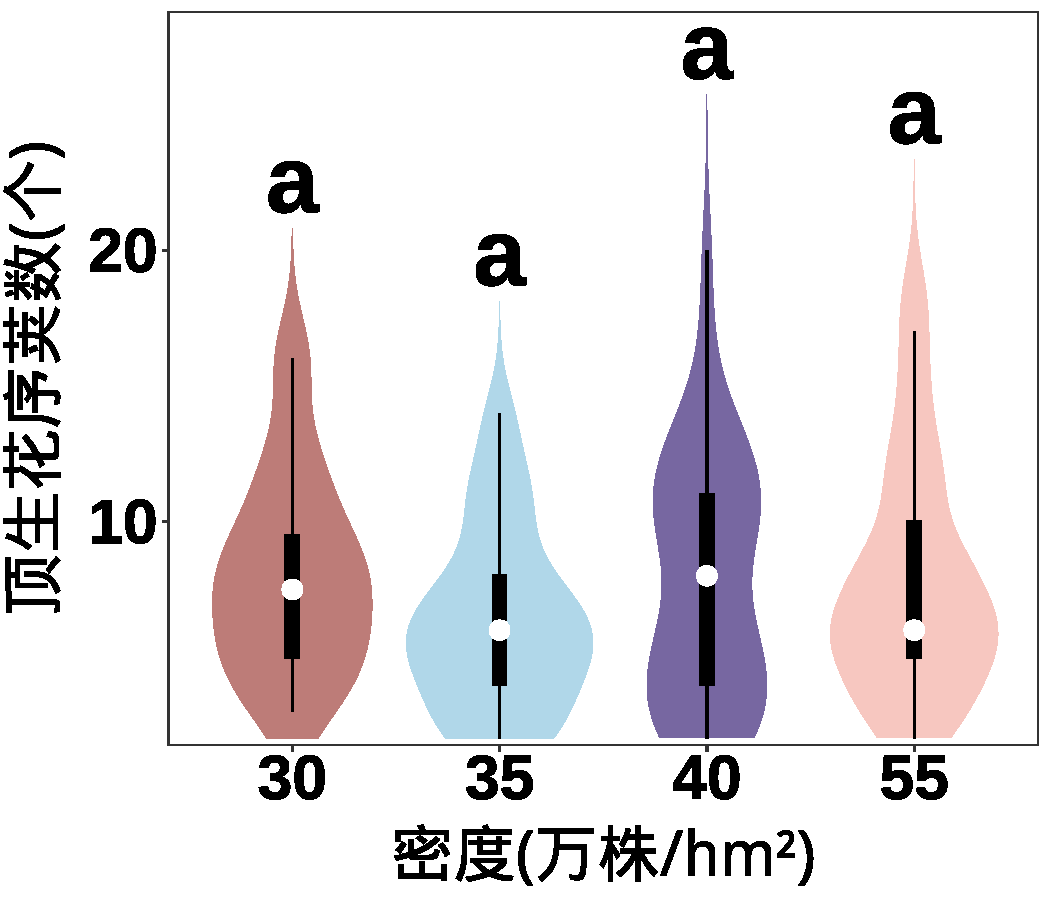
\includegraphics[width=0.24\linewidth]{Figure/2025/bar/PTR}
		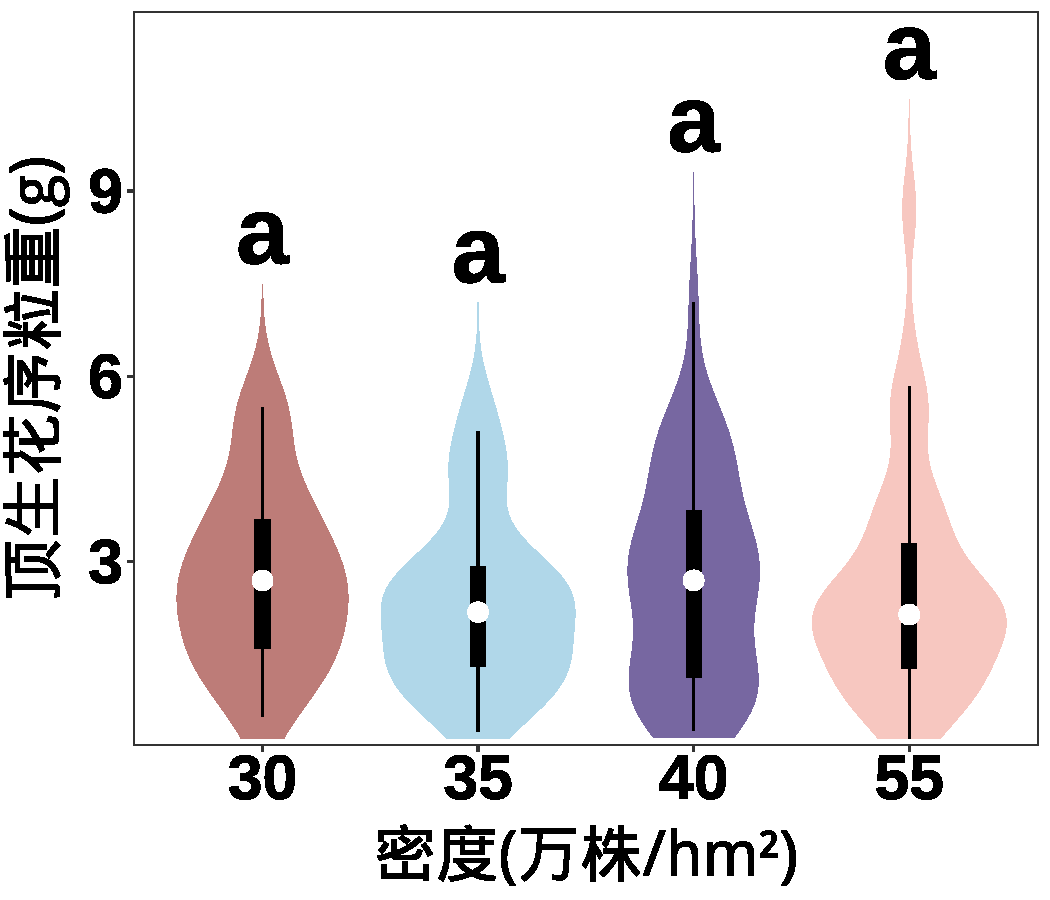
\includegraphics[width=0.24\linewidth]{Figure/2025/bar/TRW}
		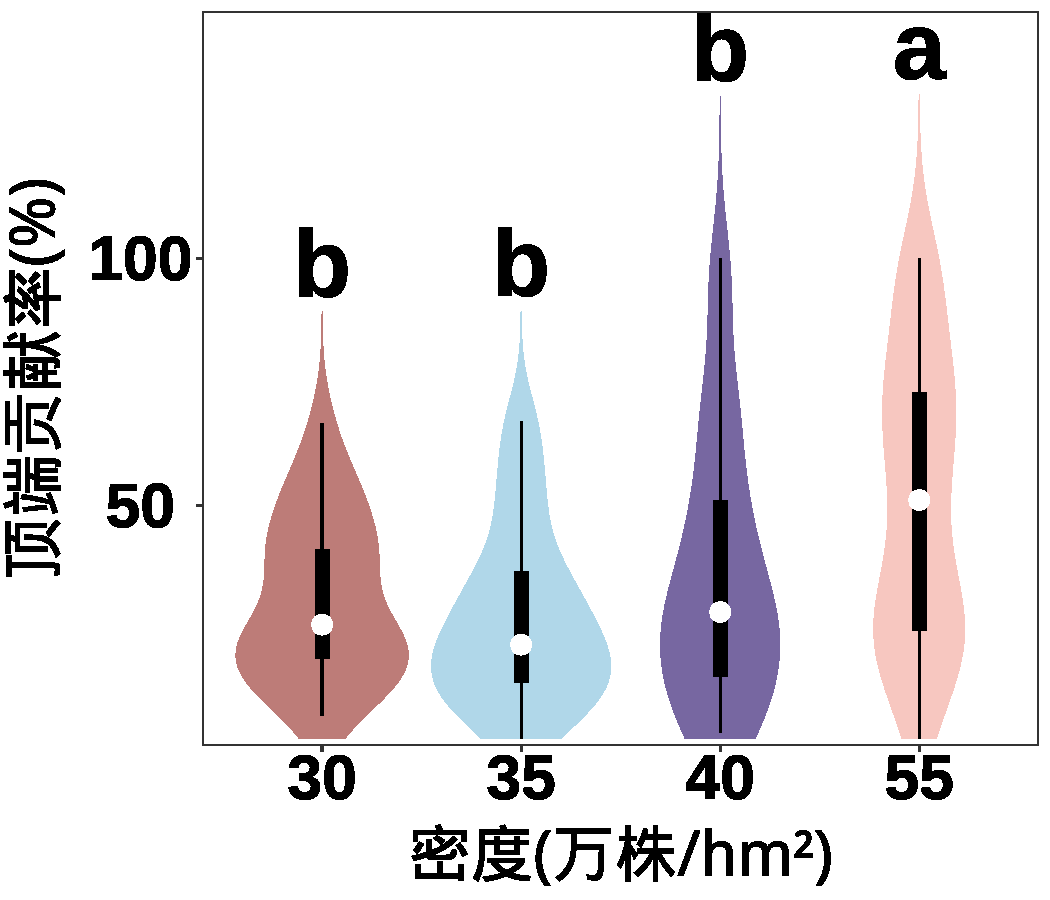
\includegraphics[width=0.24\linewidth]{Figure/2025/bar/CTRY}
		\caption{不同种植密度下 LFI297 农艺性状变化}
		\label{fig:duochongbijiao}
		\footnotesize A 中属于 2024 年，B 中属于 2025 年。不同小写字母表示不同处理间差异显著($P < 0.05$)。图中的白点为中位数。
	\end{figure}
			
	\chapter{讨论}

	基于第三章系统分析的试验结果，本章从多个角度对种植密度调控扁茎大豆后代稳定品系 LFI297 个体发育与群体产量的内在机制进行深入探讨，并结合前人研究对试验结果的科学意义与实践价值进行综合评价。
	
	\section{种植密度对LFI297个体发育与群体产量的调控效应}
	
	种植密度作为协调作物个体生长与群体发展的关键栽培措施，其调控效应在大豆生产实践中具有重要意义\cite{Lv2008}。本研究连续两年的试验结果表明，随着种植密度的增加，扁茎大豆后代稳定品系 LFI297 的群体产量呈现出先显著上升后逐渐下降的非线性变化规律，回归模型拟合显示该响应曲线符合二次多项式模型（2024 年 $R^2 = 0.716^*$）。这一结果与 Gan 等\cite{Gan2002,xu2021}的研究相符：大豆群体产量的形成本质上是群体库容扩大与个体源供应衰退之间的博弈。在适宜密度范围内（如 2025 年 LFI297 的 30--35 万株/hm$^2$），增加密度能增大群体库容；但越过临界阈值后，个体的过度荫蔽和分枝大量减少将引发群体产量的下降。
	
	在 2024 年的试验中，当密度从 24 万株/hm$^2$增加至 34 万株/hm$^2$时，产量提升了 34.8\%，34 万株/hm$^2$处理的群体产量达到最高，为 5067.18 kg/hm$^2$；结合 2024 年综合评价结果，30 万株/hm$^2$处理综合排序第二，34 万株/hm$^2$综合排序第一。在 2025 年进一步细化密度梯度的试验中，35 万株/hm$^2$处理的综合表现最优（产量和综合评价排序第一），40 万株/hm$^2$产量和综合排序第二，30 万株/hm$^2$综合排序第三。综合两年数据表明，扁茎大豆后代稳定品系 LFI297 在吉林省中部的最适宜种植密度区间为 30--40 万株/hm$^2$。在近似的产量峰值密度下（35 万株/hm$^2$左右），2025 该大豆品系产量较 2024 年有所下降，这可能与 2025 年生育后期田间病害的发生、2024 年和 2025 年大豆全生育期降雨量的差异（2025 年比 2024 年高 144.3 mm）有关。
		
	\chapter{结论}

	本研究连续两年的田间试验与系统分析，针对扁茎大豆后代稳定品系 LFI297 在不同种植密度下的个体发育、群体产量形成机制及品质特征，得出以下主要结论：

	% 以下为正文之后的部分，默认不进行章节编号。
	% heading=bibintoc    : 将参考文献加入目录中
	% heading=bibnumbered : 参考文献列表参与章节
	\normalem
	\printbibliography[heading = bibintoc]

	% 各附录。
	% \appendix
	% \chapter{}
	% % \section{TODO}
	% 目前由Tex Live2020生成的文件存在页眉中章节号变为英文的问题。
	% 推荐在安装Tex Live时取消选择自动更新。
	% 我们致力于解决此问题，欢迎各位同学沟通解决方案。
	% 此问题预计将会在下一个版本中修复。
	% \chapter{}

	\backmatter	
	%  \chapter{作者简介及科研成果}
	% 	\section*{作者简介}
	% 	学姐，女，汉族，1995年1月1日出生于**省**市。
	% 	A本科就读于吉林大学计算机科学与技术专业，硕士就读于吉林大学科学与技术专业，主要研究方向为***。

	% 	\section*{科研成果}
	% 	\vskip 10pt
	% 	\begin{itemize}[itemsep= 7pt, labelsep= 10pt, leftmargin = 25pt, topsep = 10pt]
	% 		\small
	% 		\setlength{\baselineskip}{16pt}
	% 		\item[{$\left[1\right]$}]
	% 		Authors. \textit{"Paper name"} [C]. In: \textit{Conference name}, \textbf{Year}, pages-pages.  doi: \texttt{doi}. (EI Accession number: \texttt{accession number}).
			
	% 		\item[{$\left[2\right]$}]
	% 		Authors. "\textit{Paper name}" [J]. \textit{Journal name}, \textbf{Year}. doi: \texttt{doi}. (CCF C类期刊).
	% 	\end{itemize}		

	\chapter{致谢}

	写之前有好多想说或者是能说的，写的时候却是说不完的，文字的力量是有限的，有好多感觉和感情是文字所无法表达出来的，但我还是想以此聊表心意。

\end{document}
